\documentclass[11pt,a4paper]{article}

\usepackage[utf8]{inputenc}
\usepackage[T1]{fontenc}
\usepackage{geometry}
\usepackage{graphicx}
\usepackage{booktabs}
\usepackage{longtable}
\usepackage{array}
\usepackage{xcolor}
\usepackage{listings}
\usepackage{tikz}
\usepackage{hyperref}
\usepackage{fancyhdr}
\usepackage{titlesec}
\usepackage{enumitem}
\usepackage{caption}
\usepackage{amsmath}
\usepackage{float}

\geometry{margin=1in}

% Define colors
\definecolor{headerblue}{RGB}{0,82,147}
\definecolor{lightgray}{RGB}{245,245,245}
\definecolor{codegray}{RGB}{240,240,240}

% Listings configuration for assembly
\lstdefinelanguage{ledasm}{
    morekeywords={ldx,ldy,cpx,cpy,inx,iny,dex,dey,bne,beq,bmi,bpl,jmp,sty,stx,stall,nop},
    sensitive=false,
    morecomment=[l]{;},
    morestring=[b]",
}

\lstset{
    basicstyle=\ttfamily\small,
    backgroundcolor=\color{codegray},
    frame=single,
    breaklines=true,
    captionpos=b,
}

% Header/Footer
\pagestyle{fancy}
\fancyhf{}
\fancyhead[L]{\textbf{LED Controller Module}}
\fancyhead[R]{Datasheet v1.0}
\fancyfoot[C]{\thepage}

% Title formatting
\titleformat{\section}
    {\Large\bfseries\color{headerblue}}
    {\thesection}{1em}{}
\titleformat{\subsection}
    {\large\bfseries\color{headerblue}}
    {\thesubsection}{1em}{}

\begin{document}

% Title Page
\begin{titlepage}
    \centering
    \vspace*{2cm}
    {\Huge\bfseries\color{headerblue} LED Controller Module\\[0.5cm]}
    {\Large Programmable SK6812RGBW LED Driver\\[0.3cm]}
    {\large with Microprogram Architecture\\[2cm]}

    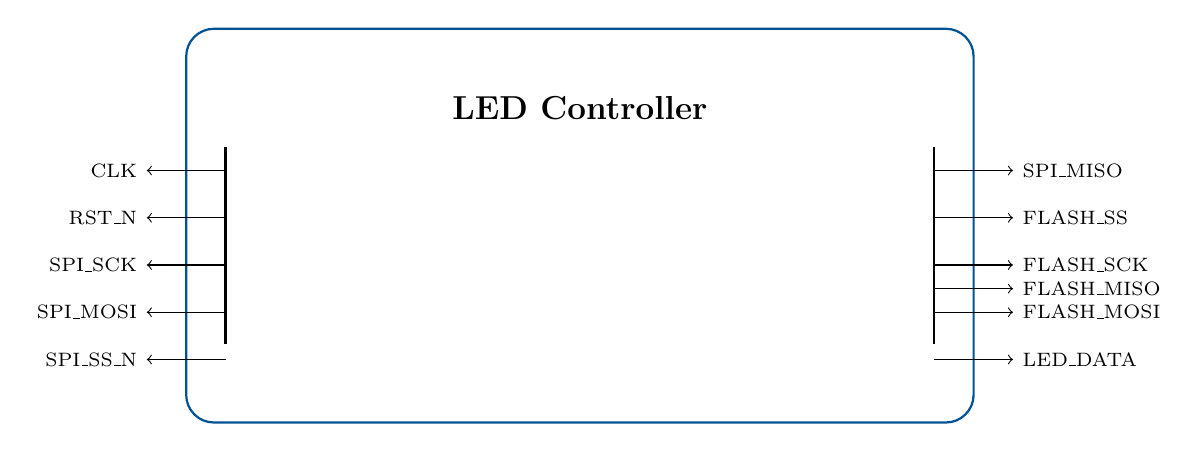
\begin{tikzpicture}
        \draw[thick, headerblue, rounded corners=10pt] (0,0) rectangle (10,5);
        \node at (5,4) {\large\textbf{LED Controller}};
        \draw[thick] (0.5,1) -- (0.5,3.5);
        \draw[thick] (9.5,1) -- (9.5,3.5);
        % Input pins
        \foreach \y/\txt in {3.2/CLK, 2.6/RST\_N, 2.0/SPI\_SCK, 1.4/SPI\_MOSI, 0.8/SPI\_SS\_N} {
            \draw[<-] (-0.5,\y) -- (0.5,\y);
            \node[left] at (-0.5,\y) {\scriptsize\txt};
        }
        % Output pins
        \foreach \y/\txt in {3.2/SPI\_MISO, 2.6/FLASH\_SS, 2.0/FLASH\_SCK, 1.4/FLASH\_MOSI, 0.8/LED\_DATA} {
            \draw[->] (9.5,\y) -- (10.5,\y);
            \node[right] at (10.5,\y) {\scriptsize\txt};
        }
        % Flash input
        \draw[<-] (10.5,1.7) -- (9.5,1.7);
        \node[right] at (10.5,1.7) {\scriptsize FLASH\_MISO};
    \end{tikzpicture}

    \vfill
    {\large Technical Datasheet\\[0.5cm]}
    {\normalsize Document Version 1.0\\}
    {\normalsize\today}
\end{titlepage}

\tableofcontents
\newpage

%==============================================================================
\section{Overview}
%==============================================================================

The LED Controller is a fully programmable SK6812RGBW LED strip driver designed for the Tiny Tapeout platform. It features a custom 8-bit microprocessor architecture that reads programs from external SPI flash memory, enabling complex LED animations without hardware modifications.

\subsection{Key Features}

\begin{itemize}[noitemsep]
    \item SK6812RGBW LED protocol support (32-bit GRBW format)
    \item Configurable LED count (up to 255 LEDs)
    \item Up to 3 configurable colors (96 bits total)
    \item Built-in LED effects: None, Chase, Pulse
    \item Custom microprogram execution from SPI flash
    \item SPI slave interface for runtime configuration
    \item Configurable clock divider for various system frequencies
    \item Chip ID: \texttt{0x6925}
\end{itemize}

\subsection{Applications}

\begin{itemize}[noitemsep]
    \item Decorative LED lighting
    \item Status indicators
    \item Custom animations and displays
    \item Wearable electronics
    \item Interactive art installations
\end{itemize}

%==============================================================================
\section{Pin Description}
%==============================================================================

\begin{table}[H]
\centering
\caption{Pin Description}
\begin{tabular}{@{}llcp{6cm}@{}}
\toprule
\textbf{Pin Name} & \textbf{Direction} & \textbf{Active} & \textbf{Description} \\
\midrule
\multicolumn{4}{l}{\textit{System Signals}} \\
\texttt{i\_clk} & Input & -- & System clock (default 50MHz) \\
\texttt{i\_reset\_n} & Input & Low & Active-low asynchronous reset \\
\midrule
\multicolumn{4}{l}{\textit{SPI Slave Interface (Configuration)}} \\
\texttt{i\_spi\_sck} & Input & -- & SPI clock \\
\texttt{i\_spi\_mosi} & Input & -- & SPI Master Out, Slave In \\
\texttt{i\_spi\_ss\_n} & Input & Low & SPI slave select (active low) \\
\texttt{o\_spi\_miso} & Output & -- & SPI Master In, Slave Out \\
\midrule
\multicolumn{4}{l}{\textit{SPI Flash Interface (Program Memory)}} \\
\texttt{o\_flash\_spi\_ss\_n} & Output & Low & Flash chip select \\
\texttt{o\_flash\_spi\_mosi} & Output & -- & Flash data output \\
\texttt{o\_flash\_spi\_sck} & Output & -- & Flash SPI clock \\
\texttt{i\_flash\_spi\_miso} & Input & -- & Flash data input \\
\midrule
\multicolumn{4}{l}{\textit{LED Output}} \\
\texttt{o\_data} & Output & -- & SK6812RGBW serial data output \\
\bottomrule
\end{tabular}
\end{table}

\subsection{Tiny Tapeout Pinout}

The following tables show the mapping of signals to Tiny Tapeout pins.

\begin{table}[H]
\centering
\caption{Dedicated Inputs (ui\_in)}
\begin{tabular}{@{}clp{6cm}@{}}
\toprule
\textbf{Pin} & \textbf{Signal} & \textbf{Description} \\
\midrule
ui[0] & SPI\_SCK & SPI slave clock \\
ui[1] & SPI\_SS\_N & SPI slave select (active low) \\
ui[2] & SPI\_MOSI & SPI slave data in \\
ui[3] & FLASH\_MISO & SPI flash data out \\
ui[4--7] & -- & Unused \\
\bottomrule
\end{tabular}
\end{table}

\begin{table}[H]
\centering
\caption{Dedicated Outputs (uo\_out)}
\begin{tabular}{@{}clp{6cm}@{}}
\toprule
\textbf{Pin} & \textbf{Signal} & \textbf{Description} \\
\midrule
uo[0] & FLASH\_SS\_N & SPI flash chip select (active low) \\
uo[1] & FLASH\_MOSI & SPI flash data in \\
uo[2] & FLASH\_SCK & SPI flash clock \\
uo[3] & LED\_DATA & SK6812RGBW serial data output \\
uo[4--7] & -- & Unused \\
\bottomrule
\end{tabular}
\end{table}

\begin{table}[H]
\centering
\caption{Bidirectional IOs (uio)}
\begin{tabular}{@{}cllp{5cm}@{}}
\toprule
\textbf{Pin} & \textbf{Signal} & \textbf{Direction} & \textbf{Description} \\
\midrule
uio[0] & SPI\_MISO & Output & SPI slave data out (active when SS\_N low) \\
uio[1--7] & -- & Input & Unused \\
\bottomrule
\end{tabular}
\end{table}

%==============================================================================
\section{SPI Register Interface}
%==============================================================================

The LED Controller exposes a register-based interface over SPI for runtime configuration. The SPI interface operates in Mode 0 (CPOL=0, CPHA=0).

\subsection{SPI Protocol}

\begin{itemize}[noitemsep]
    \item \textbf{Read}: Send register address (bit 7 = 0), receive data on next byte
    \item \textbf{Write}: Send register address with bit 7 = 1, then send data byte
    \item Auto-increment addressing for consecutive reads/writes
\end{itemize}

\subsection{Register Map}

\begin{table}[H]
\centering
\caption{Register Map}
\begin{tabular}{@{}cclcl@{}}
\toprule
\textbf{Addr} & \textbf{Name} & \textbf{R/W} & \textbf{Default} & \textbf{Description} \\
\midrule
0x01 & EFFECT & R/W & 0x03 & Active effect (see below) \\
0x02 & CHIP\_ID\_H & R & 0x69 & Chip ID high byte \\
0x03 & CHIP\_ID\_L & R & 0x25 & Chip ID low byte \\
0x04--0x07 & COLOR0 & R/W & 0x00FF0000 & Color 0 (GRBW format) \\
0x08--0x0B & COLOR1 & R/W & 0xFF000000 & Color 1 (GRBW format) \\
0x0C--0x0F & COLOR2 & R/W & 0x0000FF00 & Color 2 (GRBW format) \\
0x10 & NUM\_LEDS & R/W & 30 & Number of LEDs (1--255) \\
0x11 & NUM\_COLORS & R/W & 3 & Number of active colors (1--3) \\
0x12 & CLK\_DIV & R/W & 5 & Clock divider for 100ns ticks \\
0x13 & FLASH\_24\_BIT & R/W & 1 & Flash address width (1=24-bit, 0=16-bit) \\
0x14 & CPU\_RESET & W & -- & Write any value to reset CPU and flash state \\
\bottomrule
\end{tabular}
\end{table}

\subsection{Effect Register Values}

\begin{table}[H]
\centering
\caption{Effect Types}
\begin{tabular}{@{}clp{8cm}@{}}
\toprule
\textbf{Value} & \textbf{Effect} & \textbf{Description} \\
\midrule
0 & NONE & Static display, all LEDs same color, cycles through colors \\
1 & CHASE & Chase animation, colors shift at 2Hz \\
2 & PULSE & Breathing/pulsing effect ($\sim$2.5 second cycle) \\
3 & CUSTOM & Execute microprogram from SPI flash \\
\bottomrule
\end{tabular}
\end{table}

\subsection{Color Format}

Colors are stored in 32-bit GRBW format (Green-Red-Blue-White):

\begin{center}
\begin{tabular}{|c|c|c|c|}
\hline
\textbf{Bits 31--24} & \textbf{Bits 23--16} & \textbf{Bits 15--8} & \textbf{Bits 7--0} \\
\hline
Green & Red & Blue & White \\
\hline
\end{tabular}
\end{center}

%==============================================================================
\section{Microprogram Architecture}
%==============================================================================

The LED Controller includes a custom 8-bit microprocessor for executing LED animation programs stored in SPI flash memory.

\subsection{CPU Specifications}

\begin{table}[H]
\centering
\caption{CPU Specifications}
\begin{tabular}{@{}ll@{}}
\toprule
\textbf{Parameter} & \textbf{Value} \\
\midrule
Data Width & 8-bit \\
Instruction Width & 16-bit (8-bit opcode + 8-bit operand) \\
Program Memory & 256 bytes (from SPI flash) \\
Scratch Memory & 16 bytes (addresses 0x10--0x1F) \\
Registers & X (8-bit), Y (8-bit), PC (8-bit) \\
Status Flags & Zero (Z), Negative (N) \\
\bottomrule
\end{tabular}
\end{table}

\subsection{Instruction Set}

\subsubsection{Load Instructions}

\begin{table}[H]
\centering
\caption{Load Instructions}
\begin{tabular}{@{}cclp{6cm}@{}}
\toprule
\textbf{Opcode} & \textbf{Binary} & \textbf{Mnemonic} & \textbf{Description} \\
\midrule
0x01 & 0001 & \texttt{ldx \#imm} & Load immediate value into X \\
0x02 & 0010 & \texttt{ldy \#imm} & Load immediate value into Y \\
0x0A & 1010 & \texttt{ldx \$addr} & Load from address into X \\
0x0B & 1011 & \texttt{ldy \$addr} & Load from address into Y \\
\bottomrule
\end{tabular}
\end{table}

\subsubsection{Store Instructions}

\begin{table}[H]
\centering
\caption{Store Instructions}
\begin{tabular}{@{}cclp{6cm}@{}}
\toprule
\textbf{Opcode} & \textbf{Binary} & \textbf{Mnemonic} & \textbf{Description} \\
\midrule
0x0E & 1110 & \texttt{sty \$addr} & Store Y to address \\
0x0F & 1111 & \texttt{stx \$addr} & Store X to address \\
\bottomrule
\end{tabular}
\end{table}

\subsubsection{Compare Instructions}

\begin{table}[H]
\centering
\caption{Compare Instructions}
\begin{tabular}{@{}cclp{6cm}@{}}
\toprule
\textbf{Opcode} & \textbf{Binary} & \textbf{Mnemonic} & \textbf{Description} \\
\midrule
0x03 & 0011 & \texttt{cpx \#imm} & Compare X with immediate \\
0x04 & 0100 & \texttt{cpy \#imm} & Compare Y with immediate \\
0x0C & 1100 & \texttt{cpx \$addr} & Compare X with address value \\
0x0D & 1101 & \texttt{cpy \$addr} & Compare Y with address value \\
\bottomrule
\end{tabular}
\end{table}

\subsubsection{Increment/Decrement Instructions}

\begin{table}[H]
\centering
\caption{Increment/Decrement Instructions}
\begin{tabular}{@{}cclp{6cm}@{}}
\toprule
\textbf{Opcode} & \textbf{Binary} & \textbf{Mnemonic} & \textbf{Description} \\
\midrule
0x05 & 0101 & \texttt{iny} & Increment Y register \\
0x06 & 0110 & \texttt{inx} & Increment X register \\
0x13 & 10011 & \texttt{dey} & Decrement Y register \\
0x14 & 10100 & \texttt{dex} & Decrement X register \\
\bottomrule
\end{tabular}
\end{table}

\subsubsection{Branch and Jump Instructions}

\begin{table}[H]
\centering
\caption{Branch and Jump Instructions}
\begin{tabular}{@{}cclp{6cm}@{}}
\toprule
\textbf{Opcode} & \textbf{Binary} & \textbf{Mnemonic} & \textbf{Description} \\
\midrule
0x07 & 0111 & \texttt{bne offset} & Branch if not equal (Z=0) \\
0x08 & 1000 & \texttt{beq offset} & Branch if equal (Z=1) \\
0x10 & 10000 & \texttt{jmp addr} & Unconditional jump (absolute) \\
0x11 & 10001 & \texttt{bmi offset} & Branch if minus (N=1) \\
0x12 & 10010 & \texttt{bpl offset} & Branch if plus (N=0) \\
\bottomrule
\end{tabular}
\end{table}

\textbf{Branch Offset Calculation:} Branch target = PC + 2 + offset. The offset is a signed 8-bit value ($-128$ to $+127$), allowing both forward and backward branches. The +2 accounts for the 16-bit instruction width.

\subsubsection{Special Instructions}

\begin{table}[H]
\centering
\caption{Special Instructions}
\begin{tabular}{@{}cclp{6cm}@{}}
\toprule
\textbf{Opcode} & \textbf{Binary} & \textbf{Mnemonic} & \textbf{Description} \\
\midrule
0x00 & 0000 & \texttt{nop} & No operation \\
0x09 & 1001 & \texttt{stall \#n} & Delay n $\times$ 10ms \\
\bottomrule
\end{tabular}
\end{table}

\subsection{Memory-Mapped Registers}

The CPU can access special hardware registers through memory addresses:

\begin{table}[H]
\centering
\caption{Memory-Mapped Hardware Registers}
\begin{tabular}{@{}clp{7cm}@{}}
\toprule
\textbf{Address} & \textbf{Name} & \textbf{Description} \\
\midrule
\$0 & \texttt{led\_count} & Number of LEDs (read-only) \\
\$1 & \texttt{color\_count} & Number of colors configured (read-only) \\
\$2 & \texttt{write\_led} & Write LED pixel (write: color index 0--2, 3=off) \\
\$10--\$1F & \texttt{scratch} & 16 bytes of scratch memory \\
\bottomrule
\end{tabular}
\end{table}

%==============================================================================
\section{SK6812RGBW Protocol}
%==============================================================================

\subsection{Timing Specifications}

The SK6812RGBW LEDs use a single-wire protocol with the following timing:

\begin{table}[H]
\centering
\caption{SK6812RGBW Timing Parameters}
\begin{tabular}{@{}llll@{}}
\toprule
\textbf{Parameter} & \textbf{Symbol} & \textbf{Typical} & \textbf{Unit} \\
\midrule
Logic 0 High Time & T0H & 300 & ns \\
Logic 0 Low Time & T0L & 900 & ns \\
Logic 1 High Time & T1H & 600 & ns \\
Logic 1 Low Time & T1L & 600 & ns \\
Reset Time & TRESET & 80 & $\mu$s \\
\bottomrule
\end{tabular}
\end{table}

\subsection{Implementation}

The \texttt{sk6812rgbw} module generates the waveform using a configurable clock divider:

\begin{itemize}[noitemsep]
    \item \textbf{Tick period}: 100ns $\times$ \texttt{clock\_divider}
    \item \textbf{Logic 0}: 3 high ticks, 9 low ticks (300ns high, 900ns low)
    \item \textbf{Logic 1}: 6 high ticks, 6 low ticks (600ns high, 600ns low)
    \item \textbf{Reset}: 800 ticks (80$\mu$s)
\end{itemize}

%==============================================================================
\section{SPI Flash Interface}
%==============================================================================

The SPI flash interface provides Execute-In-Place (XIP) functionality for the microprocessor, reading program instructions directly from external SPI flash memory.

\subsection{XIP (Execute-In-Place)}

The LED Controller implements XIP to execute programs directly from SPI flash without requiring internal program memory. This approach enables:

\begin{itemize}[noitemsep]
    \item Unlimited program size (limited only by flash capacity)
    \item Easy program updates by reprogramming the flash
    \item Minimal on-chip memory requirements
\end{itemize}

\textbf{Important:} XIP mode is \textbf{enabled by default}. On power-up, the controller immediately begins executing code from SPI flash address 0x0000. Ensure valid program code is present in flash before powering on the device.

\subsubsection{Cache Implementation (Future Enhancement)}

A cache line implementation exists in the design (\texttt{spi\_flash\_cache.sv}) with configurable cache line size and number of cache lines. However, due to area constraints on the Tiny Tapeout 2x2 tile, the cache module is not instantiated in the current build. This may be included in future larger tile implementations.

The cache parameters (when enabled) are:
\begin{itemize}[noitemsep]
    \item Cache line size: 32--64 bytes
    \item Number of cache lines: 2
    \item Total cache: 64--128 bytes (32--64 instructions)
\end{itemize}

\subsection{Flash Specifications}

\begin{table}[H]
\centering
\caption{SPI Flash Interface Parameters}
\begin{tabular}{@{}ll@{}}
\toprule
\textbf{Parameter} & \textbf{Value} \\
\midrule
SPI Mode & Mode 0 (CPOL=0, CPHA=0) \\
SPI Clock Divider & 2 (fixed, relative to system clock) \\
Maximum SPI Clock & 25 MHz (at 50 MHz system clock) \\
Read Command & 0x03 (Standard Read) \\
Address Width & 24-bit (default) or 16-bit \\
Data Width & 8-bit \\
\bottomrule
\end{tabular}
\end{table}

\textbf{Note:} The SPI flash clock operates at half the system clock frequency. At the default 50 MHz system clock, the flash SPI clock is 25 MHz. This ensures compatibility with most standard SPI flash devices which typically support 25--50 MHz operation.

\subsection{Address Width Configuration}

The flash interface supports both 16-bit and 24-bit addressing modes:

\begin{table}[H]
\centering
\caption{Flash Address Width Options}
\begin{tabular}{@{}lll@{}}
\toprule
\textbf{Mode} & \textbf{Register Value} & \textbf{Addressable Range} \\
\midrule
24-bit (default) & FLASH\_24\_BIT = 1 & 16 MB \\
16-bit & FLASH\_24\_BIT = 0 & 64 KB \\
\bottomrule
\end{tabular}
\end{table}

24-bit addressing is enabled by default to support larger flash devices. When using small flash chips (64KB or less), 16-bit mode can be enabled for slightly faster instruction fetch.

\subsection{Read Sequence}

\begin{enumerate}[noitemsep]
    \item Assert chip select (CS\_N = 0)
    \item Send read command (0x03)
    \item Send address (24-bit or 16-bit, MSB first)
    \item Receive data bytes (continuous read while CS\_N low)
    \item Deassert chip select (CS\_N = 1)
\end{enumerate}

%==============================================================================
\section{Timer System}
%==============================================================================

The LED Controller includes a hierarchical timer system:

\begin{table}[H]
\centering
\caption{Timer Configuration}
\begin{tabular}{@{}llll@{}}
\toprule
\textbf{Timer} & \textbf{Frequency} & \textbf{Period} & \textbf{Usage} \\
\midrule
Base Timer & 100 Hz & 10 ms & CPU stall timing \\
10 Hz Timer & 10 Hz & 100 ms & Pulse effect brightness steps \\
2 Hz Timer & 2 Hz & 500 ms & Chase effect \\
2s Timer & 0.5 Hz & 2 s & Long delays \\
\bottomrule
\end{tabular}
\end{table}

The base timer uses 1,000,000 clock ticks with the configured clock divider to achieve 10Hz at 50MHz system clock.

%==============================================================================
\section{Electrical Characteristics}
%==============================================================================

\subsection{Recommended Operating Conditions}

\begin{table}[H]
\centering
\caption{Recommended Operating Conditions}
\begin{tabular}{@{}lcccc@{}}
\toprule
\textbf{Parameter} & \textbf{Symbol} & \textbf{Min} & \textbf{Typ} & \textbf{Max} \\
\midrule
System Clock Frequency & $f_{CLK}$ & 10 & 50 & 100 MHz \\
Clock Divider (for 50MHz) & CLK\_DIV & -- & 5 & -- \\
Supply Voltage & VDD & 3.0 & 3.3 & 3.6 V \\
\bottomrule
\end{tabular}
\end{table}

\subsection{Clock Divider Calculation}

To achieve correct SK6812RGBW timing, set the clock divider based on system frequency:

\[
\text{CLK\_DIV} = \frac{f_{CLK} \text{ (MHz)}}{10}
\]

For example:
\begin{itemize}[noitemsep]
    \item 20 MHz: CLK\_DIV = 2
    \item 30 MHz: CLK\_DIV = 3
    \item 40 MHz: CLK\_DIV = 4
    \item 50 MHz: CLK\_DIV = 5
    \item 100 MHz: CLK\_DIV = 10
\end{itemize}

%==============================================================================
\section{Reset Behavior}
%==============================================================================

On reset, the controller initializes to the following state:

\begin{table}[H]
\centering
\caption{Default Reset Values}
\begin{tabular}{@{}ll@{}}
\toprule
\textbf{Parameter} & \textbf{Default Value} \\
\midrule
Effect Mode & CUSTOM (0x03) -- XIP enabled \\
Number of LEDs & 30 \\
Number of Colors & 3 \\
Clock Divider & 5 \\
Flash Address Width & 24-bit \\
Color 0 & 0x00FF0000 (Green) \\
Color 1 & 0xFF000000 (Red) \\
Color 2 & 0x0000FF00 (Blue) \\
CPU Program Counter & 0x00 \\
\bottomrule
\end{tabular}
\end{table}

The reset synchronizer uses a 2-stage flip-flop chain to prevent metastability issues with asynchronous reset de-assertion.

%==============================================================================
\section{Application Notes}
%==============================================================================

\subsection{Connecting SK6812RGBW LEDs}

Connect \texttt{o\_data} to the DIN pin of the first LED in the strip.

\subsection{Programming via SPI}

Example SPI write sequence to change effect to CHASE:

\begin{lstlisting}[language={},caption={SPI Write Example}]
1. Assert SS_N (low)
2. Send: 0x81 (Write to register 0x01)
3. Send: 0x01 (EFFECT_CHASE)
4. Deassert SS_N (high)
\end{lstlisting}

Example SPI read sequence to read chip ID:

\begin{lstlisting}[language={},caption={SPI Read Example}]
1. Assert SS_N (low)
2. Send: 0x02 (Read register 0x02)
3. Receive: 0x69 (CHIP_ID_H)
4. Receive: 0x25 (CHIP_ID_L, auto-increment)
5. Deassert SS_N (high)
\end{lstlisting}

\subsection{Writing Custom Programs}

\begin{enumerate}[noitemsep]
    \item Write assembly code using the instruction set
    \item Assemble to 16-bit binary (opcode:operand pairs)
    \item Program into SPI flash starting at address 0x0000
    \item Set effect mode to CUSTOM (0x03)
\end{enumerate}

%==============================================================================
\section{Revision History}
%==============================================================================

\begin{table}[H]
\centering
\caption{Document Revision History}
\begin{tabular}{@{}lll@{}}
\toprule
\textbf{Version} & \textbf{Date} & \textbf{Description} \\
\midrule
1.0 & \today & Initial release \\
\bottomrule
\end{tabular}
\end{table}

\end{document}
